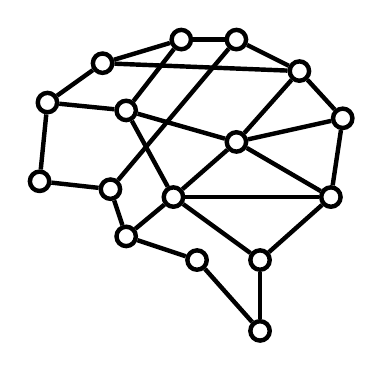
\begin{tikzpicture}
    \tikzstyle{hidden neuron}=[circle, draw, ultra thick, minimum size=7pt,inner sep=0pt];
    
    % \node[hidden neuron] (n1) at (0.5,0) {};
    \node[hidden neuron] (n2) at (1,0.3) {};
    
    \node[hidden neuron] (n3) at (0.2,1.2) {};
    \node[hidden neuron] (n4) at (1,1.2) {};
    
    \node[hidden neuron] (n5) at (1.9,2) {};
    \node[hidden neuron] (n6) at (-0.7,1.5) {};
    
    \node[hidden neuron] (n7) at (2.05,3) {};
    \node[hidden neuron] (n8) at (-0.9,2.1) {};
    
    \node[hidden neuron] (n9) at (1.5,3.6) {};
    \node[hidden neuron] (n10) at (-1.8,2.2) {};
    
    \node[hidden neuron] (n11) at (0.7,4) {};
    \node[hidden neuron] (n12) at (-1.7,3.2) {};
    
    \node[hidden neuron] (n13) at (0,4) {};
    \node[hidden neuron] (n14) at (-1,3.7) {};
    
    \node[hidden neuron] (n15) at (-0.7,3.1) {};
    \node[hidden neuron] (n16) at (0.7,2.7) {};
    \node[hidden neuron] (n17) at (-0.1,2) {};
    
    \draw[ultra thick] (n2) -- (n3);
    \draw[ultra thick] (n2) -- (n4);
    \draw[ultra thick] (n3) -- (n6);
    \draw[ultra thick] (n4) -- (n5);
    \draw[ultra thick] (n5) -- (n7);
    \draw[ultra thick] (n6) -- (n8);
    \draw[ultra thick] (n7) -- (n9);
    \draw[ultra thick] (n8) -- (n10);
    \draw[ultra thick] (n9) -- (n11);
    \draw[ultra thick] (n10) -- (n12);
    \draw[ultra thick] (n11) -- (n13);
    \draw[ultra thick] (n12) -- (n14);
    \draw[ultra thick] (n13) -- (n14);
    
    \draw[ultra thick] (n4) -- (n17);
    \draw[ultra thick] (n6) -- (n17);
    \draw[ultra thick] (n15) -- (n16);
    \draw[ultra thick] (n15) -- (n17);
    \draw[ultra thick] (n16) -- (n17);
    
    \draw[ultra thick] (n15) -- (n12);
    \draw[ultra thick] (n8) -- (n11);
    
    \draw[ultra thick] (n5) -- (n16);
    \draw[ultra thick] (n7) -- (n16);
    
    \draw[ultra thick] (n14) -- (n9);
    \draw[ultra thick] (n13) -- (n15);
    
    \draw[ultra thick] (n16) -- (n9);
    \draw[ultra thick] (n17) -- (n5);
    
\end{tikzpicture}